\chapter{Introduction}
\label{ch:Introduction}

\stress{\textbf{Disclaimer to this document:} 
This is a template with some additional thesis information and a sample structure. 
The structure includes the chapters most commonly needed in a thesis. 
Neither the order nor the chapter titles are fixed and will most likely 
have to be adapted to your specific thesis. 
However, the notes here should help you to get an idea what each chapter 
could be about and how to use this template. 
When in doubt, please talk to your supervisor(s).}

Your thesis should start with an introduction. The introduction is supposed to motivate your thesis.
Discuss the relevance of your topic, why are you looking into it, why is it relevant in the field? Cite important research related to your motivation.
Briefly state the problem as in the abstract and repeat the contribution, for example in the form of research questions. 

Give an outline of your thesis.

Testing the glossaries package \gls{rmse}


Below, you will find an example figure (\Cref{fig:example}). Please use the caption of your figures to describe everything in the figure, additionally to what you have written about the figure in the text. Everyone should be able to understand the figure just reading its caption.

\begin{figure}[h!]%
\centering
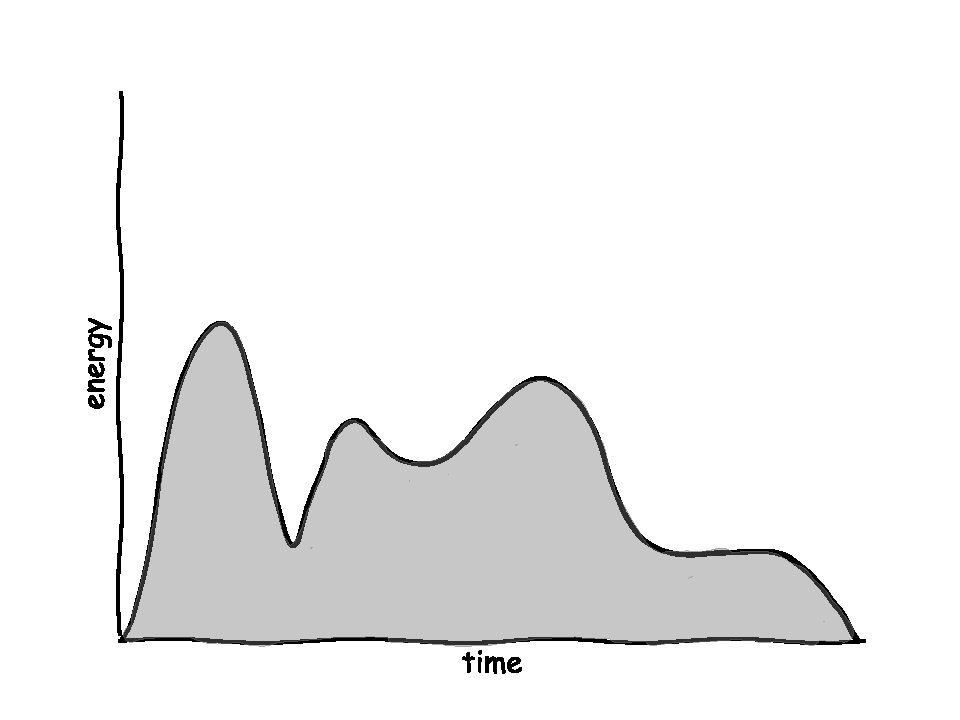
\includegraphics[width=0.5\columnwidth]{plots/Figure_2_demand}%
\caption{This is an example figure. It shows a fictional demand of energy (in grey) over time.}%
\label{fig:example}%
\end{figure}

\section{The GEFCom2014 Dataset}
\label{sec:gefcom-dataset}

In order to compare different energy forecasting methods, 
\Textcite{Hong2016} organized the Global Energy Forecasting Competition 2014 (GEFCom2014), 
a probabilistic energy forecasting competition with four tracks: 
electric load, electric price, wind power and solar power forecasting. 
The competition attracted 581 participants from 61 countries. 

The Global Energy Forecasting Competition took place the first time in 2012. 
In the 2014 competition, they upgraded the competition with three features: 
\begin{enumerate}
    \item instead of point forecasts, probabilistic forecasts were used;
    \item four forecasting tracks were used: electric load (L track), 
    electric price (P track), wind power (W track) and solar power (S track);
    \item incremental data releases on a weekly basis to mimic real world forecasting.
\end{enumerate}

In this thesis, we will only look at the solar power track. 
In this track, the task is to predict the power generation of three 
solar power plants (the so called zones) in Australia. 
The prediction is on a rolling basis for \(\SI{24}{\hour}\) ahead. 
The forecasts are to be issued at midnight each day for the next \(24\) hours. 
\(15\) tasks are provided for the challenge. In each one, the participants need to 
provide one month of forecasts, so \(28\)-\(31\) days.
For the forecasts, different prediction variables from the 
European Centre for Medium-Range Weather Forecasts (ECMWF) are provided. 
They are shown in Table \ref{table:predictors}.
Power measurements are also provided, but only over the training period. 

In order to become familiar with the data, only the last twelve of the 15 available tasks 
from April 2013 to June 2014 counted towards the final score.
The final score was calculated using a linear increasing weighted mean over the scores from the different tasks: 
The first task got weight \(1/78\), the second \(2/78\), etc. 
in order to promote models that improve over time. The division by \(78\) is so that the 
weights sum to \(1\).
Since we will evaluate the models on the dataset as a whole instead of on a monthly different basis, 
we will take the mean over the \(12\) different losses.

\begin{table}[ht]
\caption[Predictors for the GEFCom2014-S track]{Predictors for the GEFCom2014-S track \par Adapted from Table 10 in \cite{Hong2016}}
\label{table:predictors}
\rowcolors{2}{white}{gray!25}
\footnotesize
\begin{tabularx}{\textwidth}{llX}
    \toprule
    \tableheads Variable name & \tableheads Units & \tableheads Comments \\
    \midrule
    Total column liquid water (tclw) & \(\si{\kilo\gram\per\square\metre}\) & Vertical integral of cloud liquid water content \\
    Total column ice water (tciw) & \(\si{\kilo\gram\per\square\metre}\) & Vertical integral of cloud ice water content \\
    Surface pressure (SP) & \(\si{\pascal}\) & \\
    Relative humidity at \(\SI{1000}{\milli\barsi}\) (r) & \(\%\) & Relative humidity is defined with respect to saturation of
                                                                  the mixed phase, i.e., with respect to saturation over ice
                                                                  below \(\SI{-23}{\degreeCelsius}\) and with respect to saturation over water 
                                                                  above \(\SI{0}{\degreeCelsius}\). In the regime in between, a quadratic
                                                                  interpolation is applied. \\
    Total cloud cover (TCC) & \(0\)-\(1\) & TCC derived from model levels using the
                                            model's overlap assumption \\
    \(10\)-metre \(U\) wind component (\(10u\)) & \(\si{\metre\per\second}\) & \\
    \(10\)-metre \(V\) wind component (\(10v\)) & \(\si{\metre\per\second}\) & \\
    \(2\)-metre temperature (\(2T\)) & \(\si{\kelvin}\) & \\
    Surface solar rad down (SSRD) & \(\si{\joule\per\square\metre}\) & Accumulated field \\
    Surface thermal rad down (STRD) & \(\si{\joule\per\square\metre}\) & Accumulated field \\
    Top net solar rad (TSR) & \(\si{\joule\per\square\metre}\) & Net solar radiation at the top of the atmosphere. Accumulated field \\
    Total precipitation (TP) & \(\si{\metre}\) & Convective precipitation \(+\) stratiform precipitation (CP + LSP). Accumulated field \\
    \bottomrule
\end{tabularx}
\end{table}